\documentclass[11pt]{article}

% Typography and Layout
\usepackage[margin=1in]{geometry}
\usepackage{microtype}
\usepackage{parskip}

% Math
\usepackage{amsmath,amssymb,amsthm}
\usepackage{mathtools}
\usepackage{bm}

% Colors and Styling
\usepackage[dvipsnames,svgnames]{xcolor}
\usepackage{tcolorbox}
\tcbuselibrary{theorems,skins,breakable}

% Graphics
\usepackage{tikz}
\usetikzlibrary{calc,patterns,angles,quotes,arrows.meta,decorations.pathmorphing,backgrounds,positioning,fit,shapes.geometric}

% Fonts
\usepackage{libertine}
\usepackage[libertine]{newtxmath}

% Custom Colors
\definecolor{theoremblue}{RGB}{45,85,145}
\definecolor{definitiongreen}{RGB}{35,120,75}
\definecolor{exampleorange}{RGB}{200,100,30}
\definecolor{lawred}{RGB}{160,50,50}
\definecolor{accentgold}{RGB}{180,140,50}
\definecolor{wavepurple}{RGB}{120,60,150}

% Theorem Environments
\newtcbtheorem[number within=section]{theorem}{Theorem}{
  enhanced,
  colback=theoremblue!8,
  colframe=theoremblue,
  fonttitle=\bfseries,
  attach boxed title to top left={yshift=-2mm,xshift=5mm},
  boxed title style={colback=theoremblue,sharp corners},
  sharp corners,
  top=4mm,
}{thm}

\newtcbtheorem[number within=section]{definition}{Definition}{
  enhanced,
  colback=definitiongreen!8,
  colframe=definitiongreen,
  fonttitle=\bfseries,
  attach boxed title to top left={yshift=-2mm,xshift=5mm},
  boxed title style={colback=definitiongreen,sharp corners},
  sharp corners,
  top=4mm,
}{def}

\newtcbtheorem[number within=section]{law}{Law}{
  enhanced,
  colback=lawred!8,
  colframe=lawred,
  fonttitle=\bfseries,
  attach boxed title to top left={yshift=-2mm,xshift=5mm},
  boxed title style={colback=lawred,sharp corners},
  sharp corners,
  top=4mm,
}{law}

\newtcbtheorem[number within=section]{principle}{Principle}{
  enhanced,
  colback=wavepurple!8,
  colframe=wavepurple,
  fonttitle=\bfseries,
  attach boxed title to top left={yshift=-2mm,xshift=5mm},
  boxed title style={colback=wavepurple,sharp corners},
  sharp corners,
  top=4mm,
}{princ}

% Title Styling
\usepackage{titlesec}
\titleformat{\section}{\Large\bfseries\color{theoremblue}}{\thesection}{1em}{}[\color{theoremblue}\titlerule]

\title{\color{theoremblue}\Huge\bfseries The Beauty of Science\\[0.3em]\large\color{gray}A Visual Journey Through Mathematics \& Physics}
\author{Demo Document}
\date{\today}

\begin{document}
\maketitle

%==============================================================================
% PART I: MATHEMATICS
%==============================================================================

\section{The Fundamental Theorem of Calculus}

\begin{theorem}{Fundamental Theorem of Calculus}{}
Let $f$ be continuous on $[a,b]$ and let $F$ be an antiderivative of $f$. Then:
\begin{equation}
  \int_a^b f(x) \, dx = F(b) - F(a)
\end{equation}
\end{theorem}

\begin{center}
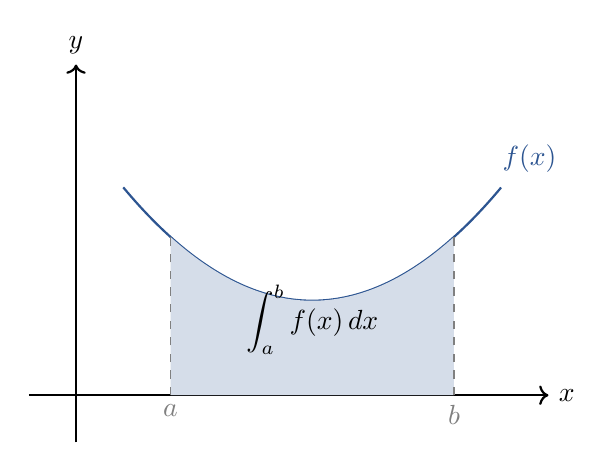
\begin{tikzpicture}[scale=1.2]
  \draw[->,thick] (-0.5,0) -- (5,0) node[right] {$x$};
  \draw[->,thick] (0,-0.5) -- (0,3.5) node[above] {$y$};
  \draw[thick,theoremblue,domain=0.5:4.5,samples=100] plot (\x,{0.3*(\x-2.5)^2+1});
  \node[theoremblue] at (4.8,2.5) {$f(x)$};
  \fill[theoremblue!20,domain=1:4,samples=100] (1,0) -- plot (\x,{0.3*(\x-2.5)^2+1}) -- (4,0) -- cycle;
  \draw[dashed,gray] (1,0) node[below] {$a$} -- (1,{0.3*(1-2.5)^2+1});
  \draw[dashed,gray] (4,0) node[below] {$b$} -- (4,{0.3*(4-2.5)^2+1});
  \node at (2.5,0.8) {$\displaystyle\int_a^b f(x)\,dx$};
\end{tikzpicture}
\end{center}

\section{Euler's Identity}

\begin{definition}{The Most Beautiful Equation}{}
Euler's identity connects five fundamental constants of mathematics:
\begin{equation}
  \boxed{\Large e^{i\pi} + 1 = 0}
\end{equation}
\end{definition}

\begin{center}
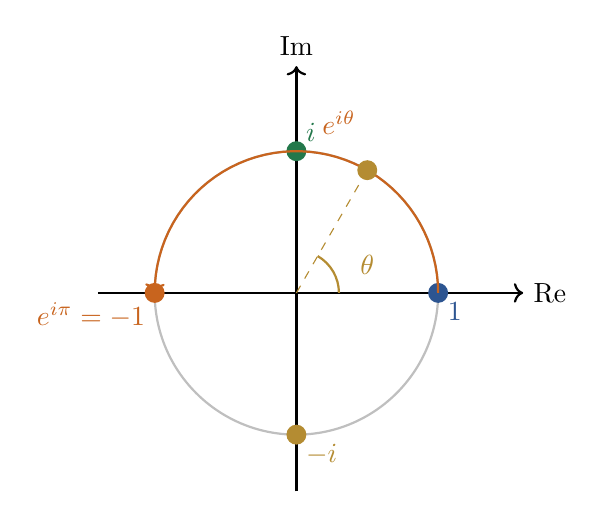
\begin{tikzpicture}[scale=1.8]
  \draw[thick,gray!50] (0,0) circle (1);
  \draw[->,thick] (-1.4,0) -- (1.6,0) node[right] {Re};
  \draw[->,thick] (0,-1.4) -- (0,1.6) node[above] {Im};
  \fill[theoremblue] (1,0) circle (2pt) node[below right] {$1$};
  \fill[exampleorange] (-1,0) circle (2pt) node[below left] {$e^{i\pi}=-1$};
  \fill[definitiongreen] (0,1) circle (2pt) node[above right] {$i$};
  \fill[accentgold] (0,-1) circle (2pt) node[below right] {$-i$};
  \draw[->,thick,exampleorange,domain=0:180,samples=50] plot ({cos(\x)},{sin(\x)});
  \node[exampleorange] at (0.3,1.2) {$e^{i\theta}$};
  \draw[thick,accentgold] (0.3,0) arc (0:60:0.3);
  \node[accentgold] at (0.5,0.2) {$\theta$};
  \fill[accentgold] ({cos(60)},{sin(60)}) circle (2pt);
  \draw[dashed,accentgold] (0,0) -- ({cos(60)},{sin(60)});
\end{tikzpicture}
\end{center}

\section{Linear Transformations}

\begin{definition}{Matrix Transformation}{}
A $2\times 2$ matrix transforms vectors in the plane:
\begin{equation}
  \underbrace{\begin{pmatrix} a & b \\ c & d \end{pmatrix}}_{\text{transformation}}
  \underbrace{\begin{pmatrix} x \\ y \end{pmatrix}}_{\text{input}} =
  \underbrace{\begin{pmatrix} ax + by \\ cx + dy \end{pmatrix}}_{\text{output}}
\end{equation}
\end{definition}

\begin{center}
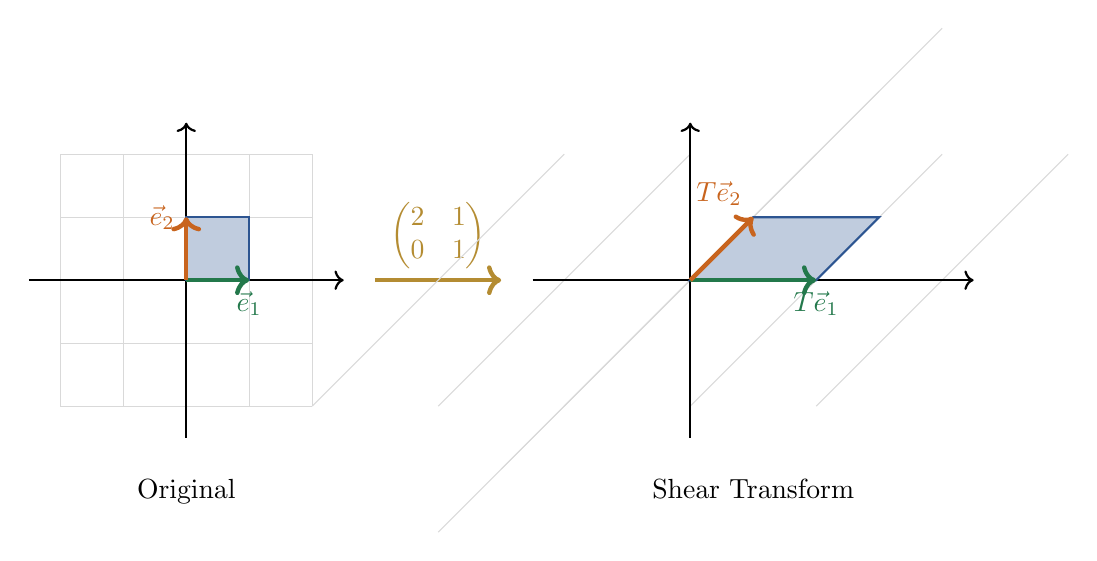
\begin{tikzpicture}[scale=0.8]
  \begin{scope}
    \draw[gray!30,step=1] (-2,-2) grid (2,2);
    \draw[->,thick] (-2.5,0) -- (2.5,0);
    \draw[->,thick] (0,-2.5) -- (0,2.5);
    \fill[theoremblue!30] (0,0) -- (1,0) -- (1,1) -- (0,1) -- cycle;
    \draw[theoremblue,thick] (0,0) -- (1,0) -- (1,1) -- (0,1) -- cycle;
    \draw[->,ultra thick,definitiongreen] (0,0) -- (1,0) node[below] {$\vec{e}_1$};
    \draw[->,ultra thick,exampleorange] (0,0) -- (0,1) node[left] {$\vec{e}_2$};
    \node[below] at (0,-3) {Original};
  \end{scope}
  \draw[->,ultra thick,accentgold] (3,0) -- (5,0) node[midway,above] {$\begin{pmatrix} 2 & 1 \\ 0 & 1 \end{pmatrix}$};
  \begin{scope}[xshift=8cm]
    \foreach \i in {-2,-1,0,1,2} {
      \draw[gray!30] ({2*\i-2},-2) -- ({2*\i+2},2);
      \draw[gray!30] ({\i-2},{\i-2}) -- ({\i+2},{\i+2});
    }
    \draw[->,thick] (-2.5,0) -- (4.5,0);
    \draw[->,thick] (0,-2.5) -- (0,2.5);
    \fill[theoremblue!30] (0,0) -- (2,0) -- (3,1) -- (1,1) -- cycle;
    \draw[theoremblue,thick] (0,0) -- (2,0) -- (3,1) -- (1,1) -- cycle;
    \draw[->,ultra thick,definitiongreen] (0,0) -- (2,0) node[below] {$T\vec{e}_1$};
    \draw[->,ultra thick,exampleorange] (0,0) -- (1,1) node[above left] {$T\vec{e}_2$};
    \node[below] at (1,-3) {Shear Transform};
  \end{scope}
\end{tikzpicture}
\end{center}

%==============================================================================
% PART II: PHYSICS
%==============================================================================

\section{Newton's Laws of Motion}

\begin{law}{Newton's Second Law}{}
The acceleration of an object is proportional to the net force:
\begin{equation}
  \boxed{\vec{F} = m\vec{a} = m\frac{d^2\vec{r}}{dt^2}}
\end{equation}
\end{law}

\begin{center}
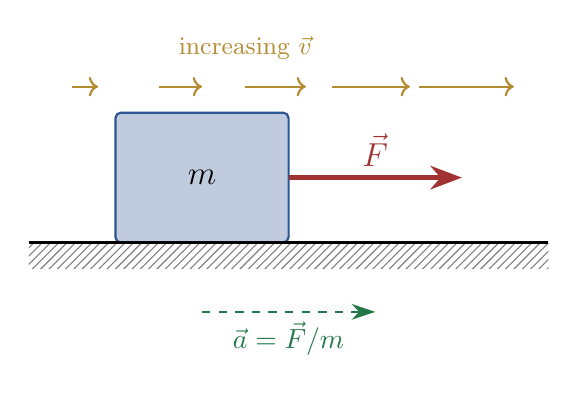
\begin{tikzpicture}[scale=1.1]
  \fill[theoremblue!30,rounded corners=2pt] (0,0) rectangle (2,1.5);
  \draw[thick,theoremblue,rounded corners=2pt] (0,0) rectangle (2,1.5);
  \node at (1,0.75) {\large $m$};
  \fill[pattern=north east lines,pattern color=gray] (-1,-0.3) rectangle (5,0);
  \draw[thick] (-1,0) -- (5,0);
  \draw[-{Stealth[length=4mm,width=3mm]},ultra thick,lawred] (2,0.75) -- (4,0.75) node[above,midway] {\large $\vec{F}$};
  \draw[-{Stealth[length=3mm,width=2mm]},thick,definitiongreen,dashed] (1,-0.8) -- (3,-0.8) node[below,midway] {$\vec{a} = \vec{F}/m$};
  \foreach \x/\len in {-0.5/0.3, 0.5/0.5, 1.5/0.7, 2.5/0.9, 3.5/1.1} {
    \draw[->,accentgold,thick] (\x,1.8) -- ({\x+\len},1.8);
  }
  \node[accentgold,above] at (1.5,2) {\small increasing $\vec{v}$};
\end{tikzpicture}
\end{center}

\section{Maxwell's Equations}

\begin{law}{Electromagnetism}{}
The four equations governing all electromagnetic phenomena:
\begin{align}
  \nabla \cdot \vec{E} &= \frac{\rho}{\epsilon_0} & &\text{\small (Gauss's Law)}\\[0.3em]
  \nabla \cdot \vec{B} &= 0 & &\text{\small (No Monopoles)}\\[0.3em]
  \nabla \times \vec{E} &= -\frac{\partial \vec{B}}{\partial t} & &\text{\small (Faraday)}\\[0.3em]
  \nabla \times \vec{B} &= \mu_0\vec{J} + \mu_0\epsilon_0\frac{\partial \vec{E}}{\partial t} & &\text{\small (Ampère-Maxwell)}
\end{align}
\end{law}

\begin{center}
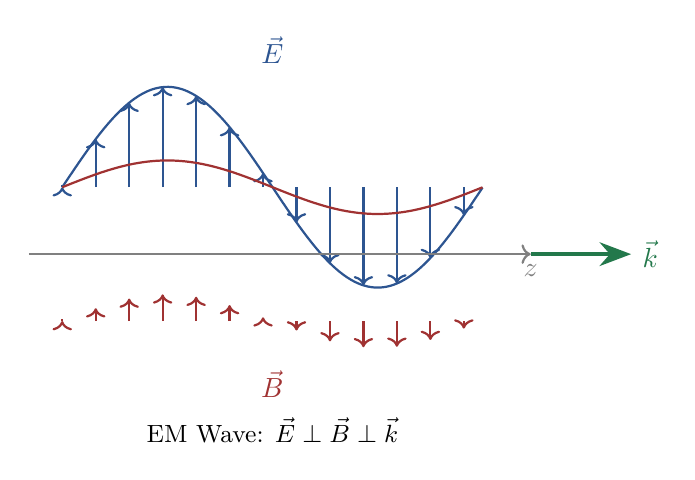
\begin{tikzpicture}[scale=0.85]
  \draw[thick,theoremblue,domain=0:6.28,samples=100,smooth] plot (\x,{1.5*sin(\x r)});
  \foreach \x in {0,0.5,...,6} {
    \draw[->,theoremblue,thick] (\x,0) -- (\x,{1.5*sin(\x r)});
  }
  \node[theoremblue,above] at (3.14,1.7) {$\vec{E}$};
  \draw[thick,lawred,domain=0:6.28,samples=100,smooth] plot (\x,{0.8*sin(\x r)*0.5}) [yshift=-2cm];
  \begin{scope}[yshift=-2cm]
    \foreach \x in {0,0.5,...,6} {
      \pgfmathsetmacro{\yval}{0.8*sin(\x r)*0.5}
      \draw[->,lawred,thick] (\x,0) -- (\x,\yval);
    }
  \end{scope}
  \node[lawred,below] at (3.14,-2.6) {$\vec{B}$};
  \draw[-{Stealth[length=4mm]},ultra thick,definitiongreen] (7,-1) -- (8.5,-1) node[right] {$\vec{k}$};
  \draw[->,thick,gray] (-0.5,-1) -- (7,-1) node[below] {$z$};
  \node[below] at (3.14,-3.3) {\small EM Wave: $\vec{E} \perp \vec{B} \perp \vec{k}$};
\end{tikzpicture}
\end{center}

\section{Special Relativity}

\begin{principle}{Mass-Energy Equivalence (Einstein, 1905)}{}
\begin{equation}
  \boxed{\Large E = mc^2}
\end{equation}
\end{principle}

\begin{center}
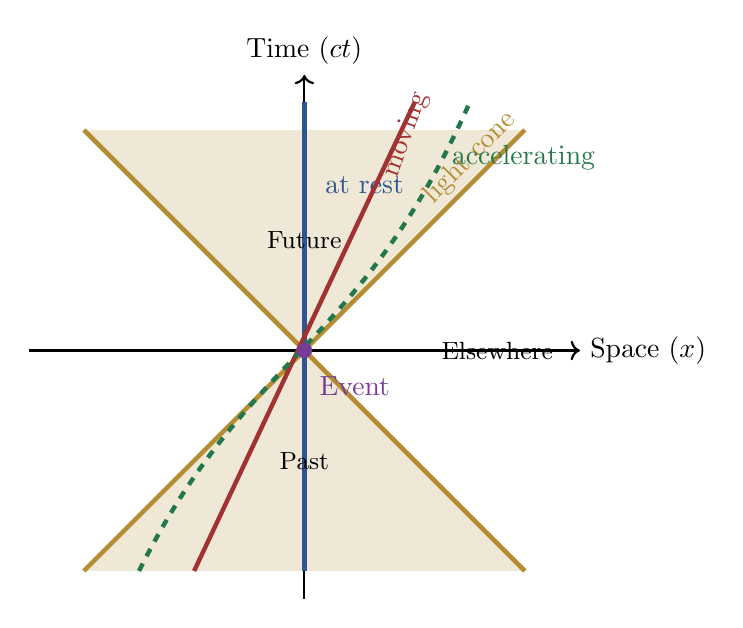
\begin{tikzpicture}[scale=0.7]
  \fill[accentgold!20] (0,0) -- (-4,4) -- (4,4) -- cycle;
  \fill[accentgold!20] (0,0) -- (-4,-4) -- (4,-4) -- cycle;
  \draw[->,thick] (-5,0) -- (5,0) node[right] {Space ($x$)};
  \draw[->,thick] (0,-4.5) -- (0,5) node[above] {Time ($ct$)};
  \draw[ultra thick,accentgold] (-4,-4) -- (0,0) -- (4,4);
  \draw[ultra thick,accentgold] (4,-4) -- (0,0) -- (-4,4);
  \node[accentgold,rotate=45] at (3,3.5) {light cone};
  \draw[ultra thick,theoremblue] (0,-4) -- (0,4.5);
  \node[theoremblue,right] at (0.2,3) {at rest};
  \draw[ultra thick,lawred] (-2,-4) -- (2,4.5);
  \node[lawred,right,rotate=70] at (1.5,3) {moving};
  \draw[ultra thick,definitiongreen,dashed] (-3,-4) .. controls (-1,0) and (1,0) .. (3,4.5);
  \node[definitiongreen,right] at (2.5,3.5) {accelerating};
  \node at (0,2) {\small Future};
  \node at (0,-2) {\small Past};
  \node at (3.5,0) {\small Elsewhere};
  \fill[wavepurple] (0,0) circle (4pt);
  \node[wavepurple,below right] at (0.1,-0.3) {Event};
\end{tikzpicture}
\end{center}

\section{The Golden Ratio}

\begin{theorem}{Divine Proportion}{}
\begin{equation}
  \varphi = \frac{1 + \sqrt{5}}{2} \approx 1.618\ldots \qquad\text{with}\qquad \lim_{n\to\infty} \frac{F_{n+1}}{F_n} = \varphi
\end{equation}
\end{theorem}

\begin{center}
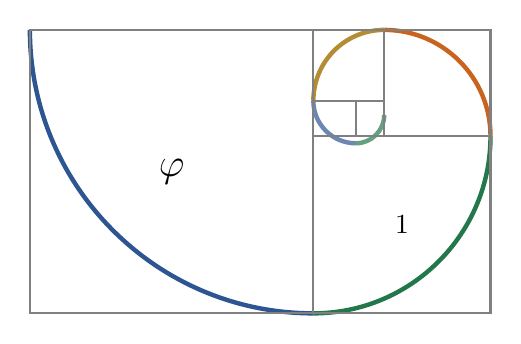
\begin{tikzpicture}[scale=0.45]
  \draw[ultra thick,theoremblue] (0,0) arc (180:270:8);
  \draw[ultra thick,definitiongreen] (8,-8) arc (270:360:5);
  \draw[ultra thick,exampleorange] (13,-3) arc (0:90:3);
  \draw[ultra thick,accentgold] (10,0) arc (90:180:2);
  \draw[ultra thick,theoremblue!70] (8,-2) arc (180:270:1.2);
  \draw[ultra thick,definitiongreen!70] (9.2,-3.2) arc (270:360:0.8);
  \draw[thick,gray] (0,0) rectangle (13,-8);
  \draw[thick,gray] (8,0) -- (8,-8);
  \draw[thick,gray] (8,-3) -- (13,-3);
  \draw[thick,gray] (10,-3) -- (10,0);
  \draw[thick,gray] (8,-2) -- (10,-2);
  \draw[thick,gray] (9.2,-2) -- (9.2,-3);
  \node at (4,-4) {\Large $\varphi$};
  \node at (10.5,-5.5) {$1$};
\end{tikzpicture}
\end{center}

\vfill
\begin{center}
\begin{tcolorbox}[colback=accentgold!10,colframe=accentgold,width=0.85\textwidth]
\centering\large\itshape
``The book of nature is written in the language of mathematics.''\\[0.3em]
\normalsize --- Galileo Galilei
\end{tcolorbox}
\end{center}

\end{document}
